\documentclass{sigchi}

%% EXAMPLE BEGIN -- HOW TO OVERRIDE THE DEFAULT COPYRIGHT STRIP -- (July 22, 2013 - Paul Baumann)
% \toappear{Permission to make digital or hard copies of all or part of this work for personal or classroom use is      granted without fee provided that copies are not made or distributed for profit or commercial advantage and that copies bear this notice and the full citation on the first page. Copyrights for components of this work owned by others than ACM must be honored. Abstracting with credit is permitted. To copy otherwise, or republish, to post on servers or to redistribute to lists, requires prior specific permission and/or a fee. Request permissions from permissions@acm.org. \\
% {\emph{CHI'14}}, April 26--May 1, 2014, Toronto, Canada. \\
% Copyright \copyright~2014 ACM ISBN/14/04...\$15.00. \\
% DOI string from ACM form confirmation}
%% EXAMPLE END -- HOW TO OVERRIDE THE DEFAULT COPYRIGHT STRIP -- (July 22, 2013 - Paul Baumann)

\toappear{}

% Arabic page numbers for submission.  Remove this line to eliminate
% page numbers for the camera ready copy 

\pagenumbering{arabic}

% Load basic packages
\usepackage{balance}  % to better equalize the last page
\usepackage{graphics} % for EPS, load graphicx instead 
\usepackage[T1]{fontenc}
\usepackage{txfonts}
\usepackage{times}    % comment if you want LaTeX's default font
\usepackage[pdftex]{hyperref}
\usepackage{url}      % llt: nicely formatted URLs
\usepackage{color}
\usepackage{textcomp}
\usepackage{booktabs}
\usepackage{ccicons}
\usepackage{todonotes}
\usepackage{pgf}
\usepackage{tikz}
\usepackage{tkz-graph}
\usepackage{mathtools}
\usepackage{amsmath}
\usepackage{algorithm}
\usepackage{algpseudocode}

% llt: Define a global style for URLs, rather that the default one
\makeatletter
\def\url@leostyle{%
  \@ifundefined{selectfont}{\def\UrlFont{\sf}}{\def\UrlFont{\small\bf\ttfamily}}}
\makeatother
\urlstyle{leo}

% To make various LaTeX processors do the right thing with page size.
\def\pprw{8.5in}
\def\pprh{11in}
\special{papersize=\pprw,\pprh}
\setlength{\paperwidth}{\pprw}
\setlength{\paperheight}{\pprh}
\setlength{\pdfpagewidth}{\pprw}
\setlength{\pdfpageheight}{\pprh}

% Make sure hyperref comes last of your loaded packages, to give it a
% fighting chance of not being over-written, since its job is to
% redefine many LaTeX commands.
\definecolor{linkColor}{RGB}{6,125,233}
%\hypersetup{%
%  pdftitle={SIGCHI Conference Proceedings Format},
%  pdfauthor={LaTeX},
%  pdfkeywords={SIGCHI, proceedings, archival format},
%  bookmarksnumbered,
%  pdfstartview={FitH},
%  colorlinks,
%  citecolor=black,
%  filecolor=black,
%  linkcolor=black,
%  urlcolor=linkColor,
%  breaklinks=true,
%}

% create a shortcut to typeset table headings
% \newcommand\tabhead[1]{\small\textbf{#1}}

\GraphInit[vstyle=Dijkstra]
\tikzset{
  EdgeStyle/.append style={->,bend left}
}

\hyphenation{PeerMind}

\begin{document}

\title{PeerMind: Towards Collective Decision-Making}

%\numberofauthors{3}
%\author{%
%  \alignauthor{1st Author Name\\
%    \affaddr{Affiliation}\\
%    \affaddr{City, Country}\\
%    \email{e-mail address}}\\
%  \alignauthor{2nd Author Name\\
%    \affaddr{Affiliation}\\
%    \affaddr{City, Country}\\
%    \email{e-mail address}}\\
%  \alignauthor{3rd Author Name\\
%    \affaddr{Affiliation}\\
%    \affaddr{City, Country}\\
%    \email{e-mail address}}\\
%}

\maketitle

\begin{abstract}

%\todo[inline]{TODO}

\end{abstract}

%\keywords{Authors' choice; of terms; separated; by semi\-colons;
%  commas, within terms only; this section is required.}

%\category{H.5.m.}{Information Interfaces and Presentation
%  (e.g. HCI)}{Miscellaneous} \category{See
%  \url{http://acm.org/about/class/1998/} for the full list of ACM
%  classifiers. This section is required.}{}{}

\section{Introduction}

Two of the most shocking democratic votes in recent history occurred in 2016:
The referendum vote for Britain to leave the European Union (``Brexit'') and the election of Donald Trump as
President of the United States.
Both votes were decided by the slimmest of margins, but more significantly, both votes had poor turnout.
We often hear that the Achilles heel of a democracy is low engagement, but this is a fallacy~---~in fact, our goal
should be to decrease engagement.
The ideal governance system is one where citizens do not have to be constantly involved, but the system is still
acting as the citizens would like it to. Can we increase legitimacy within a democracy while also decreasing the
attention required at the same time?

In this paper we present our work on improving the collective decision-making through use of a web application
to facilitate the process.
In contrast with existing similar solutions, our web application integrates new ideas in how to improve this process:
use of range voting, dynamic quorum, and vote delegation.
The broad idea is that instead of just trying to move the voting process online~---~something many others have done
previously~---~we in fact wish to add value by voting online.
Specifically, we can compute results faster, more accurately,
%and securely,
we can use sophisticated statistics to
estimate important quantities for the entire voting population, we can allow for members to entrust others who have
more expertise on topics than they do themselves, and we can promote clarity and full understanding of the voting
items for all.

%The broad idea is that instead of just trying to move the voting process online -- something many others do -- we in
%fact add additional value by voting online.
%Specifically, we can compute results faster and more accurately, we can use sophisticated statistics to estimate
%quantities for the entire voting population, and we can promote clarity and full understanding of the voting items for all.
%
%\todo[inline]{Main questions and answers follow.}
%
%What problem are we solving? Why is it important to solve? What is the story?
%
%Finding a way to lower attention required but increase legitimacy of democratic decisions.
%Traditionally legitimacy is increased by increasing participation/attention required.
%It is an everlasting problem.
%How to outsource governance and at the same time assure it does not get corrupt
%or tyrannic.
%
%Has anyone else tried to solve it or related problems? How did they try
%and what were the results (subjective or objective)?
%
%Described here: \url{http://mitar.tnode.com/post/73983101095/peer-to-peer-voting-scheme}.
%Some tried delegations, but mostly only to one person.
%Getting issues that you have tree-structure with possible cycles you cannot resolve.
%Often there were reported UI problems as well.
%So just technically improving is not enough, you also have to have UI for the technical solution so that people can trust.
%
%How are you solving the problem? What technologies are you using?
%
%Using dynamic quorum, range voting, delegation, and nice integration with UI/UX.
%
%How will you know how well you solved the problem? How will those technologies address the issues?
%
%If it improves decision making, participation, inclusivity, activity of people engaged in decision making in my house.
%So currently we have issues with reaching the quorum and many people do not participate.
%I would like for them to have easier time participating (less time required) and as a consequence more people to
%participate collectively.
%If I observe that I think I will know I solved the problem.
%
%\todo[inline]{This rest of the section is mostly notes. Organize and improve.}
%
%We can often hear that the issue of our democracy is low engagement.
%But this is a fallacy, because we should be instead trying to decrease engagement.
%The best governance system is one where you do not have to be involved yourself, but it is still doing things
%like you would like to do them.
%% Or even, doing things you might not even know that you would like to be done, especially in a long term.
%We want to outsource the job of coordination between people.
%Sometimes you want to coordinate people yourself (in your company, team), you might enjoy it, but in most cases
%you cannot or do not want to, so you outsource this service, especially at a large scale.
%
%One reason why increasing engagement sounds like a good idea is because current democratic systems have two
%questionable assumptions: participants have time to participate, and knowledge to participate.
%If you do not participate it is your fault.
%Moreover, the legitimacy of decisions is based on participation as well.
%This is why those participating in the these democratic systems have motivation to try to increase participation
%of others (especially if they believe they will still be in majority), or claim they are at fault to not participate.
%
%engagement is then increased only to assure that people like the results
%
%so if we try to minimize engagement, but still make sure that people like the results, then this is the perfect system
%
%and only in the case when they are on the loosing side, then we have to make sure that they understand the reasons why
%they lost (e.g.,\ the middle panel in our design) or at least to feel that they participated, in at least some way
%(voting, or just delegating)
%
%but the participation is the last on this list of important factors
%
%the more important thing is that they understand why others were thinking differently
%or that they do not even have to be engaged
%
%we want that people do not have to pay attention to what government is doing
%
%currently, we are in a loop where we have a useless feedback loop, where government in fact would like for people
%to pay some type of attention because they need to be elected, so they have to show like they are doing something,
%but on the other hand they do not want too much engagement, because they do not have things in place to really
%engage with everyone
%
%government should be like infrastructure, you should not have to care about it while it works, and be there to fix
%things if it starts failing, but not even you personally, but have mechanisms and processes in place to find this
%
%Terminology:
%\begin{itemize}
%\item community -- group which is making a decision using PeerMind
%\item member -- user of the app who is participating in decision making
%\end{itemize}
%
%\todo[inline]{Terminology: decision vs. vote vs. voting (how to name the step in decision making where you vote, and what is what you cast?)}
%\todo[inline]{Terminology: motion? Tally? What is the sum of all votes?}
%\todo[inline]{Terminology: discarding a vote if you didn't vote and didn't delegate. Some other term?}
%
%The main question is: can we increase legitimacy and decrease attention required at the same time.
%Many others are trying to increase attention (participation) because they want to increase legitimacy,
%assuming that this is the only way.
%
%A list of potential other points:
%\begin{itemize}
%\item legitimacy (quorum, involvement of more people through delegation)
%\item scaling (delegation helps, less attention helps)
%\item attention (at same or better decisions)
%\item bad assumptions for democracy - time, knowledge, it is rational to know that you do not know, common practice is to ask friends
%\item better decisions (more people consulted, attention directed where it should be)
%\end{itemize}
%
%Another question: should feedback be visible (to see how others voted before you voted)?
%People go with majority.
%Better for wisdom of crowds is an independent sample.
%Maybe we should only allow how other voted to be seen after you voted (but you can still change the vote),
%but we could then observe that and learn from this and see if this is good or bad.
%Or we could just store information if you observed existing votes before you voted (you have to click a button to see them).
%Maybe going with majority is also good when you want more social cohesion in the community and not so much ``optimal''
%wisdom of crowds result -  you would want that people relax their positions based on how other people care.
%Cohesion of the group vs. accuracy.
%Maybe display only number of votes and credibility, maybe credibility direction or graph, but not average votes.
%
%A list of potential questions:
%\begin{itemize}
%\item Delegation works?
%\item Statistical quorum works?
%\item Real-time feedback influences?
%\item Private vs. public delegation (do you know how member to whom you delegated is voting)?
%\item When delegating, how to assure that you cannot learn how somebody else voted, but that you can still somehow
%learn how your vote is used?
%\item Knowing how much power you have vs. not knowing -- does it change how people behave? (Knowing might corrupt you,
%but also motivate you to do more thorough work voting because you know other depend on you.)
%\end{itemize}
%
%Performance/theory/scaling in computational terms (how big could effectively community can be to be able to compute it).
%Some other theoretical properties?
%Computing statistical quorum is an ``embarrassingly parallel'' problem, and so its
%use would not suffer in large populations.
%Sparsity of delegation matrix also enables use of (recently developed?)
%efficient matrix computation algorithms.
%
%Out of scope of this work:
%
%\begin{itemize}
%\item How to assure privacy of the delegation network (it is highly sensitive data, probably even more than votes)?
%\item How to compute delegation results in a way that it does not require access to the whole network of delegation at once?
%\item How can we make this system distributed (and still assure privacy)?
%\end{itemize}
%
%\section{Related work}
%
%\cite{andersen2008trust, dirnstorfer2010voting, ford2002delegative, rodriguez2007smartocracy, yamakawa2007toward}

\section{Features}

\subsection{Range Voting}

Range voting (also known as score voting) is voting where members of a community express their positions on open proposals by assigning
each a score on a fixed scale, in the context of this paper, between $-1$ and $+1$.
A proposal passes if the average score of all votes on a position is positive.
When multiple competing proposals are being voted on, the one with highest average score wins.

Prior work has shown that this approach generalizes many previous approaches to voting and allows members to express their
positions in a highly informative and precise manner.
We find it especially suitable for a web application because many web users are used to use it when ranking products
and giving other ``five-star'' feedback.
Moreover, if later on a new proposal is added to a set of existing proposals on which voting was already open, only the
new proposal needs to be evaluated by members, as opposed to alternative voting systems where the relative rankings of
each proposal would need reassessing (assuming members use a consistent personal scale when voting).

\subsection{Dynamic Quorum}

%\todo[inline]{Unify terminology: population -> community, voters -> members, item -> proposal, motion -> proposal}

Dynamic quorum uses statistical hypothesis testing to compute the minimum number of required votes needed
to achieve a desired level of confidence before a community adopts an outcome as being truly representative of
its members' positions.
For example, in a community of 100 members, if 20 members vote in full support of a proposal, then we can conclude
with very high confidence that, had all 100 members actually voted, a majority them would support the proposal,
despite in actuality 80 members not having voted.
On the other hand, if 80 members vote but 41 vote in support of the proposal and 39 vote in opposition,
the community cannot yet conclude anything with high confidence.
Hence, the suggested action would be for the community to gather more votes and continue discussion around the proposal.
By utilizing a dynamic quorum, we can direct attention and participation of the community towards contentious proposals,
while reducing attention towards proposals which already have overwhelming support.

\subsubsection{Background}
A population of voters (a community) needs to collectively decide which item (if any) to take action on out of a set of competing items.
In order to democratically take action, the population needs to have a \{simple, super\}-majority of ``yes'' votes on a
winning item, while also demonstrating that the winning item is preferred over all other competing items.
We do not want to poll the entire population, but we do want to be certain (specifically, $99\%$ certain) that
the population does not take undesired actions, which in this case encompasses taking action on an item that is not
supported by a majority of the population and/or taking action on an item that is not clearly preferred over all
other competing alternatives.

\subsubsection{Problem Statement}
We wish to compute the probability that the bias in a population towards voting ``yes'' is greater than some
fraction of the population (e.g., $50\%$ for a simple majority, $67\%$ for a super majority).
In addition, we wish to compute the probability that the bias towards voting ``yes'' on a specific item is greater
than the bias towards voting ``yes'' on all other competing items.

\subsubsection{Assumptions}
We assume that there is a fixed underlying bias in the population that is to be estimated given raw voting data.

Without any votes, we assume that this bias may be any value between $0\%$ and $100\%$ with equal probability.

\subsubsection{Voting}
We allow for range voting where each member of the population may choose any real number in the range $[-1,+1]$ to
represent their vote, with $-1$ representing opposition and $+1$ representing support.
In the theory subsection below, we rescale votes to be in the range $[0,1]$ via the notation $\frac{votes + 1}{2}$.

We allow voters to ``abstain'' from voting.
We treat abstentions as indicating that a voter is removing themselves from the population of voters for an item.
It is important to distinguish an ``abstention'' (removing yourself from the voting population) from voting $0$
(indicating indifference).

\subsubsection{Bayesian Theory}

The commonplace and convenient choice of using the Beta distribution as our prior on the population bias is a
consequence of the Beta distribution's conjugacy with the binomial distribution, a distribution that arises
naturally when considering samples from a finite population.\footnote{To
properly understand the Bayesian approach to parameter estimation, read the following instructive tutorial:
\url{http://www.behind-the-enemy-lines.com/2008/01/are-you-bayesian-or-frequentist-or.html}
The tutorial is very similar to the problem we have at hand.}

After extracting the sufficient statistics from raw votes~---~namely the average score and the number of
abstentions~---~we can adjust the effective population size and corresponding threshold.
In addition, we can calculate the effective number of ``yes'' and ``no'' votes.\footnote{Which one can think
of as the number of Heads and Tails in the aforementioned tutorial.}

Let
\begin{description}
\begin{itemize}
\item[$C = $] $\{X_1,\ldots, X_n\}$, the set of competing motions,
\item[$N = $] population size,
\item[$X_i = $] $\{v_1, \ldots, v_{m_i}\}$, the $m_i$ raw votes for motion $X_i$, excluding ``abstentions'',
\item[$N_i = $] $(N - \textrm{number of abstentions on } X_i)$, the effective population voting on motion $X_i$,
\item[$\alpha_i = $] $\sum\limits_{v \in X_i} \left(\frac{v+1}{2}\right)$, the effective number of ``yes'' votes on motion $X_i$,
\item[$\beta_i = $] $m_i - \alpha_i$, the effective number of ``no'' votes on motion $X_i$,
\item[$K_i = $] $N_i - m_i$, the number of remaining votes yet to be cast on $X_i$,
\item[$p_i = $] true latent population bias towards voting ``yes'' on $X_i$.
\end{itemize}
\end{description}

When we have a single motion open for voting, $C=\{X_1\}$, we simply wish to compute:
\begin{align}\label{eq1}
\Pr(\alpha^*_1 > T_1 \mid X_1),
\end{align}
where
\begin{description}
\begin{itemize}
\item[$\alpha^*_i = $] the total number of ``yes'' votes for $X_i$ if we were to sample the entire population,
\item[$T_i = $] $f \cdot N_i$, for some fraction $f$ corresponding to the type of majority needed for the vote
(e.g. $f=\frac{1}{2}$ for a simple majority).
\end{itemize}
\end{description}
Using the prior $p_1 \mid X_1 \sim \operatorname{Beta}(1+\alpha_1,1+\beta_1)$, corresponding to a uniform prior when
no votes have been cast ($\alpha_1 = \beta_1 = 0$), we can express \eqref{eq1} as:
\begin{align*}
\Pr(\alpha^*_1 > T_1 \mid X_1) &= 1 - \Pr(\alpha^*_1 \leq T_1 \mid X_1),\\
\Pr(\alpha^*_1 \leq T_1 \mid X_1) &= \int_0^1 \Pr(\alpha^*_1 \leq T_1 \mid p_1)\cdot \Pr(p_1 \mid X_1) \mathrm{d}p_1\\
&= \int_0^1 \sum\limits_{i=0}^{V_1} {K_1 \choose i} p_1^{i} {(1-p_1)}^{K_1-i} \\
& \qquad\qquad\quad \times \operatorname{Beta}(p_1; 1+\alpha_1,1+\beta_1) \mathrm{d}p_1,
\end{align*}
where
\begin{description}
\begin{itemize}
\item[$V_i = $] $\lfloor{T_i - \alpha_i}\rfloor$, the maximum number of additional ``yes'' votes allowed such that
$X_i$ would remain below threshold.
\end{itemize}
\end{description}

Hence, we have
\begin{align}\label{eq2}
& \Pr(\alpha^*_1 > T_1 \mid X_1) = \nonumber\\
& 1 - \int_0^1 \sum\limits_{i=0}^{V_1} {K_1 \choose i} p_1^{i} {(1-p_1)}^{K_1-i} \cdot \operatorname{Beta}(p_1; 1+\alpha_1,1+\beta_1) \mathrm{d}p_1
\end{align}

In the scenario where $\mathbf{card}(C) = n > 1$, i.e., there are competing motions, there is additional complexity to
consider.
Without loss of generality, assume that $X_1$ is the most popular motion within $C$.
We now wish to not only compute \eqref{eq1}, but also the probability that $X_1$ is superior to all other
$X_i  \in C, i \neq 1$:

\begin{align}\label{eq3}
\Pr\left(\bigwedge_{i=2}^n (\alpha^*_1 > \alpha^*_i) \mid C\right)
\end{align}

Using the assumption
that votes on motions are independent across motions, which, in the common
scenario where there is a negative covariance between votes on competing
motions, will provide a lower bound on the probability, we can decompose \eqref{eq3} as follows:
\begin{align*}
& \Pr\left(\bigwedge_{i=2}^n (\alpha^*_1 > \alpha^*_i) \mid C\right)\\
=& \prod_{i=2}^n \Pr(\alpha^*_1 > \alpha^*_i \mid C)\\
=& \prod_{i=2}^n \iint\limits_{p_1, p_i} \Pr(\alpha^*_1 > \alpha^*_i \mid p_1, p_i) \cdot \Pr(p_1 \mid X_1) \cdot \Pr(p_i \mid X_i) \mathrm{d}p_i \mathrm{d}p_1\\
=& \prod_{i=2}^n \int_0^1 \int_0^1 \Pr(\alpha^*_1 > \alpha^*_i \mid p_1, p_i) \cdot \operatorname{Beta}(p_1; 1+\alpha_1,1+\beta_1) \\
& \qquad\qquad\qquad \times \operatorname{Beta}(p_i; 1+\alpha_i,1+\beta_i) \mathrm{d}p_i \mathrm{d}p_1\\
\end{align*}
Deriving an expression for $\Pr(\alpha^*_1 > \alpha^*_i \mid p_1, p_i)$, we get:
\begin{align*}
& \Pr(\alpha^*_1 > \alpha^*_i \mid p_1, p_i)\\
=& 1 - \Pr(\alpha^*_1 \leq \alpha^*_i \mid p_1, p_i)\\
=& 1 - \sum\limits_{m=0}^{K_1} \sum\limits_{n=\lceil{v_{1,i}+m}\rceil}^{K_i} {K_1 \choose m} p_1^{m} {(1-p_1)}^{K_1 - m} \cdot {K_i \choose n} p_i^{n} {(1-p_i)}^{K_i-n},
\end{align*}
where
\begin{description}
\begin{itemize}
\item[$v_{i,j} = $] $\alpha_i - \alpha_j$, the number of effective ``yes'' votes $X_i$ leads $X_j$ by.
\end{itemize}
\end{description}

Denoting
\begin{align}\label{eq4}
& \Phi_i(p_1,p_i) {\overset {\underset {\mathrm {def} }{}}{=}} \nonumber\\
& 1 - \sum\limits_{m=0}^{K_1} \sum\limits_{n=\lceil{v_{1,i}+m}\rceil}^{K_i} {K_1 \choose m} p_1^{m} {(1-p_1)}^{K_1 - m} \cdot {K_i \choose n} p_i^{n} {(1-p_i)}^{K_i-n},
\end{align}
we can simplify \eqref{eq3} to:
\begin{align}\label{eq5}
& \Pr\left(\bigwedge_{i=2}^n (\alpha^*_1 > \alpha^*_i) \mid C\right)\nonumber\\
&= \prod_{i=2}^n \int_0^1 \int_0^1 \Phi_i(p_1,p_i) \cdot \operatorname{Beta}(p_1; 1+\alpha_1,1+\beta_1) \nonumber\\
& \qquad\qquad\qquad \times \operatorname{Beta}(p_i; 1+\alpha_i,1+\beta_i) \mathrm{d}p_i \mathrm{d}p_1
\end{align}

We can numerically compute \eqref{eq2} and \eqref{eq5} given raw voting data.
In order to be certain before taking any actions, we would like for the computed credibilities to be $\geq 99\%$.

\begin{figure}[ht]
\centering
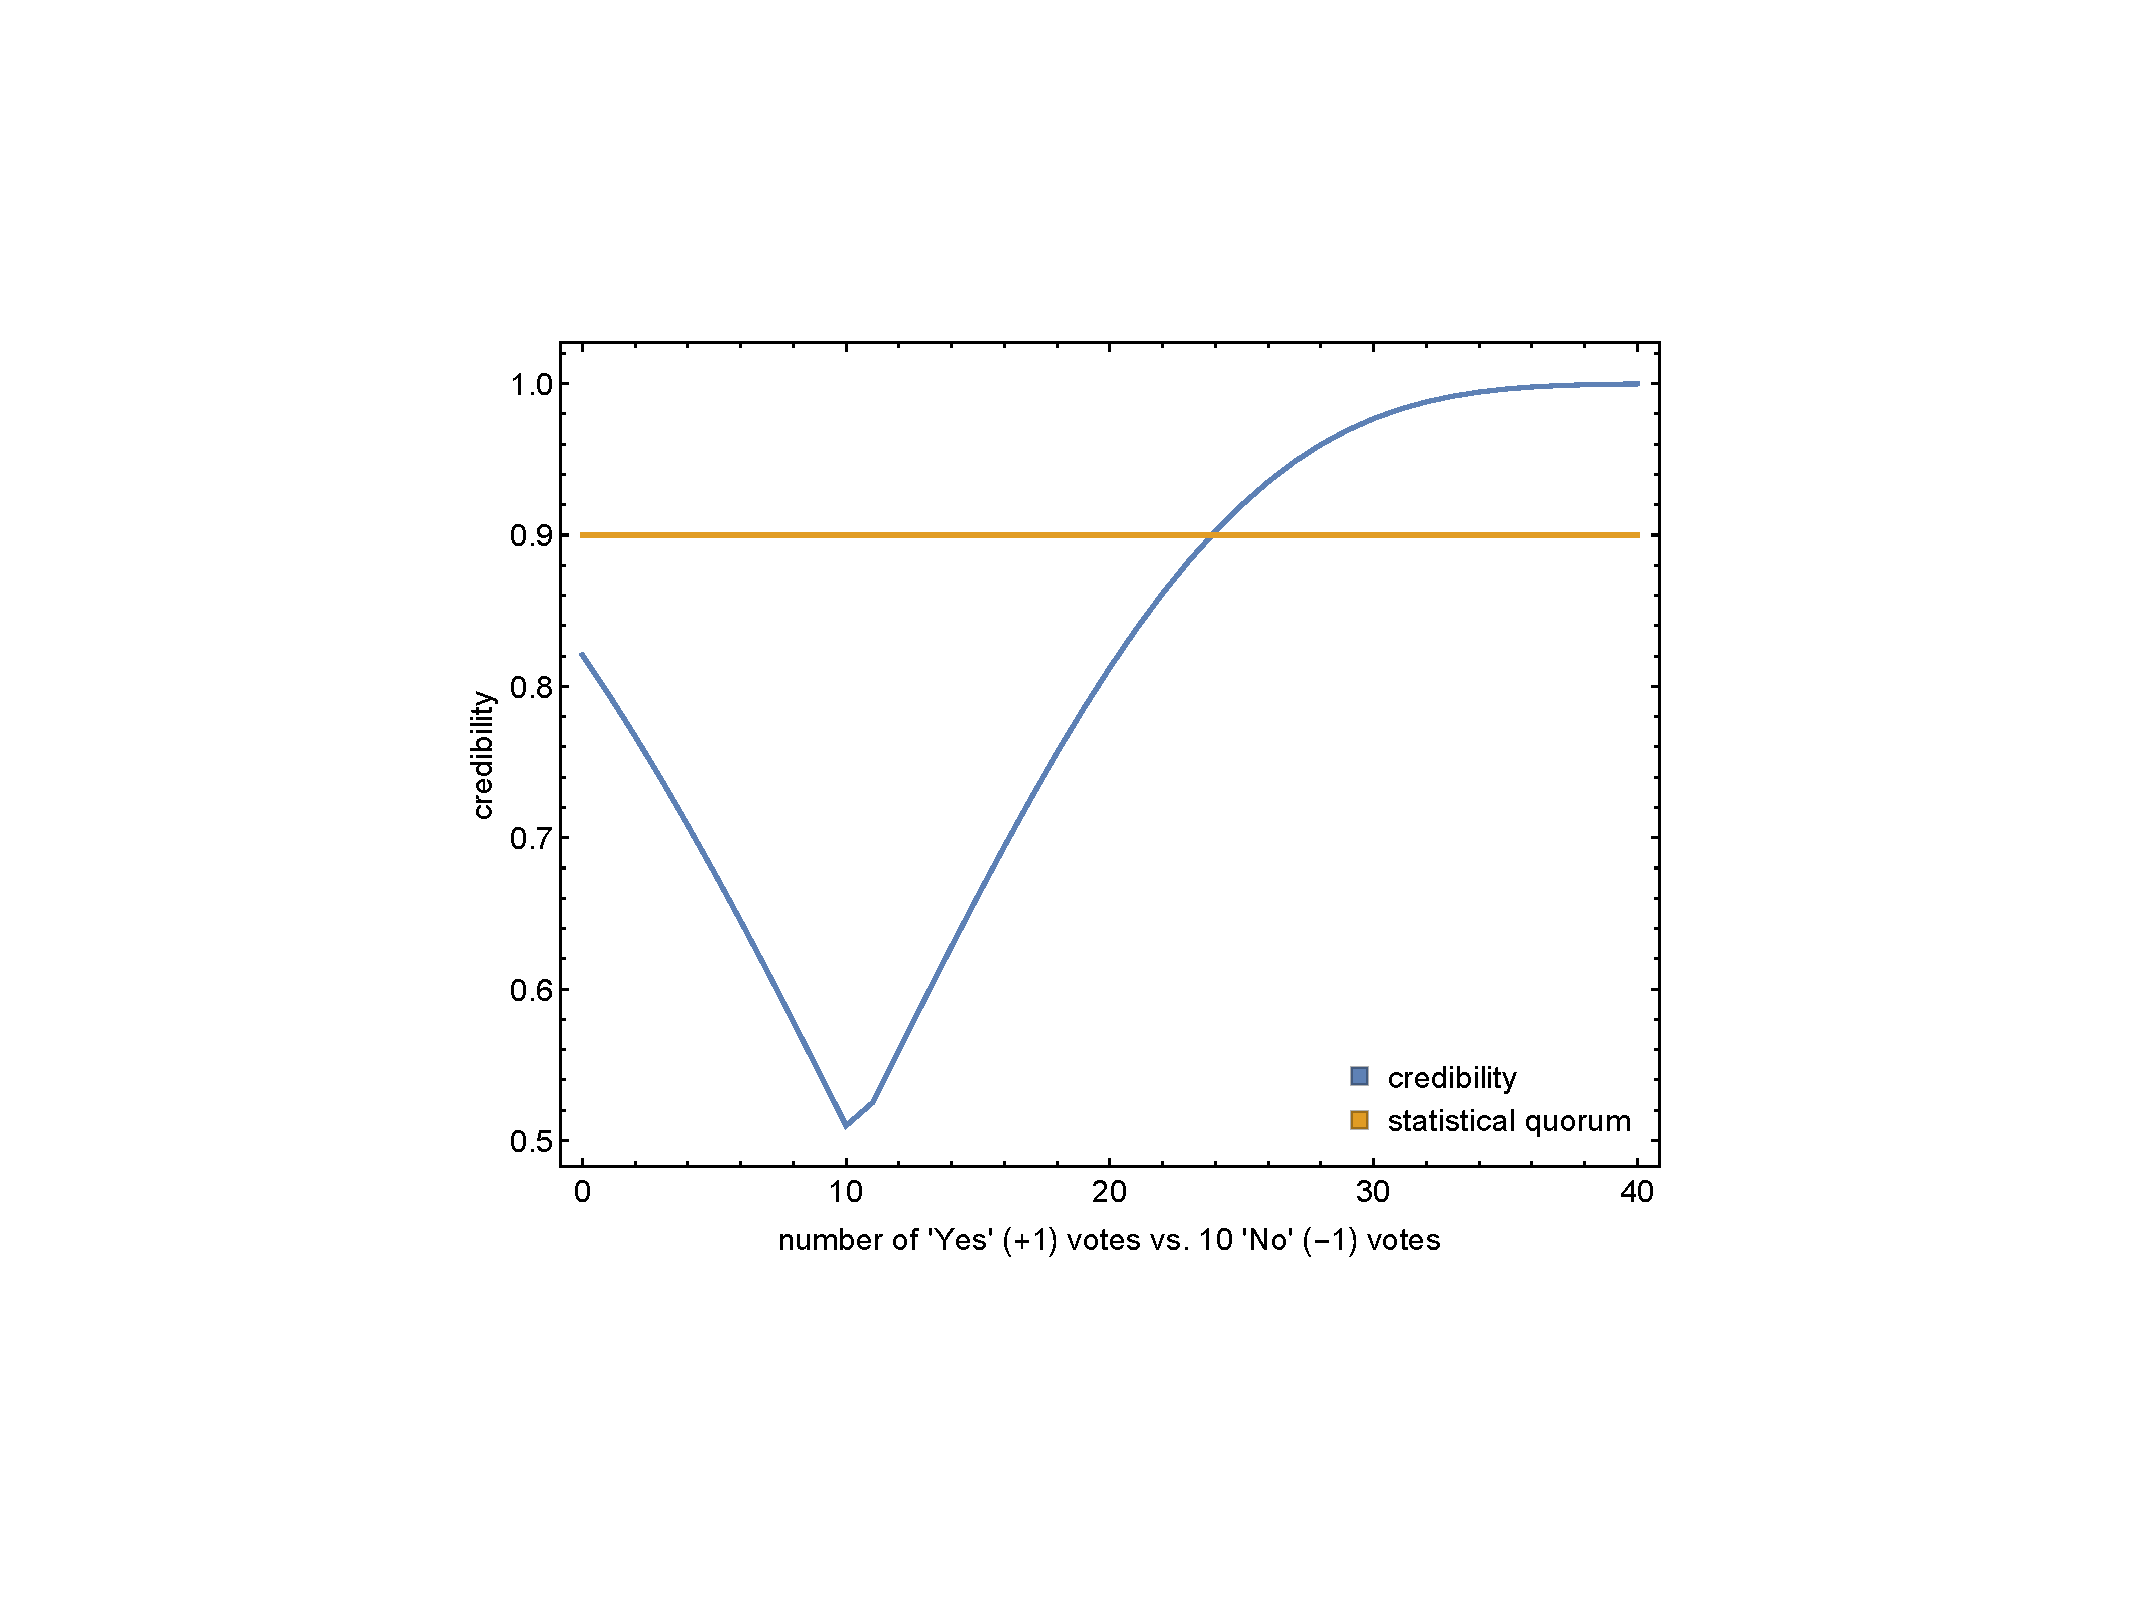
\includegraphics[width=0.5\textwidth]{figures/simple_majority}
\caption{Simple Majority: $\alpha$ vs. $\Pr(\alpha > \frac{1}{2}N)$ for $N=100$, $\beta = 10$.}
\label{simple_majority}
\end{figure}
%Data:
%Curve 1: {{0,0.000299648},{1,0.00213083},{2,0.00817989},{3,0.0224777},{4,0.049512},{5,0.0928927},{6,0.154136},{7,0.232044},{8,0.322859},{9,0.421057},{10,0.520467},{11,0.615358},{12,0.701241},{13,0.775267},{14,0.836245},{15,0.884385},{16,0.920892},{17,0.947532},{18,0.966265},{19,0.978973},{20,0.987296},{21,0.992561},{22,0.99578},{23,0.997682},{24,0.998767},{25,0.999366}}
%Curve 2: {x, 0.99} for all x

\begin{figure}[ht]
\centering
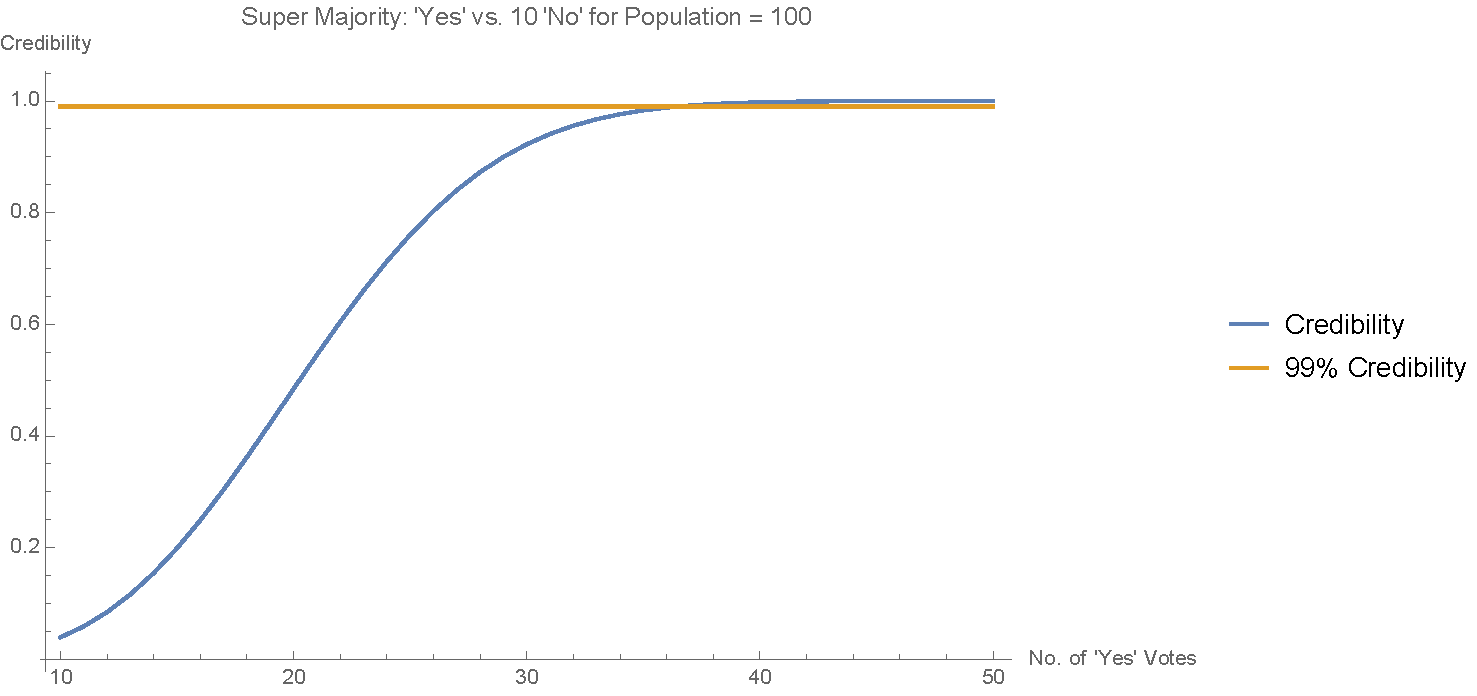
\includegraphics[width=0.5\textwidth]{figures/super_majority}
\caption{Super Majority: $\alpha$ vs. $\Pr(\alpha > \frac{2}{3}N)$ for $N=100$, $\beta = 10$.}
\label{super_majority}
\end{figure}
%Data:
%Curve 1: {{10,0.0395173},{11,0.0591278},{12,0.0846131},{13,0.116407},{14,0.15463},{15,0.199057},{16,0.24911},{17,0.303899},{18,0.362273},{19,0.422909},{20,0.484399},{21,0.545345},{22,0.604445},{23,0.660559},{24,0.712764},{25,0.760382},{26,0.802985},{27,0.840385},{28,0.872612},{29,0.899875},{30,0.922519},{31,0.940987},{32,0.955777},{33,0.967407},{34,0.976384},{35,0.983186},{36,0.988243},{37,0.99193},{38,0.994567},{39,0.996414},{40,0.997682},{41,0.998533},{42,0.999093},{43,0.999452},{44,0.999677},{45,0.999815},{46,0.999896},{47,0.999944},{48,0.99997},{49,0.999985},{50,0.999993}}
%Curve 2: {x, 0.99} for all x

%\todo[inline]{Do we take into the account the distribution of votes? So if you have a very large standard deviation
%we might want to prefer a decision less than some other decision with smaller standard deviation, but maybe
%also smaller (but still positive) average. Is distribution of votes influencing dynamic quorum?}

\subsection{Delegation}
%\todo[inline]{Max: I think delegation graph edges should point in the direction towards the person that the vote is
%being given to (more intuitive).
%\\
%Mitar: We are not giving votes to people, we are delegating a decision to people, but votes are computed for each person
%separately based on how delegates voted themselves. The idea is that you ask a delegate how the voted and then compute
%your vote. The do not get your vote to do anything with it. This is why arrows are like that. Maybe the word
%"delegation" is confusing and we should maybe use surrogate or some other word.}
Because not every member of the community has time or knowledge to vote all the time, each member can delegate
decisions to one or more other members of the community.
When a member does not vote themselves, information how those delegates voted is combined into a vote of
the non-voting member.
If a delegate has not voted themselves either, their vote is computed through delegation as well, recursively.

Each member $M$ can declare their delegates and ratios $r$ in which delegates' votes are combined. For example:

\begin{itemize}
\item Member $M_1$ decides not to delegate at all.
\item Member $M_2$ delegates to $M_1$ and $M_4$ with ratios $0.75$ ($r_{2,1}$) and $0.25$ ($r_{2,4}$), respectively.
\item Member $M_3$ delegates to $M_4$ with ratio $1.00$ ($r_{3,4}$).
\item Member $M_4$ delegates to $M_2$, $M_3$, and $M_5$ with ratios $0.40$ ($r_{4,2}$), $0.40$ ($r_{4,3}$), and $0.20$ ($r_{4,5}$), respectively.
\item Member $M_5$ decides not to delegate.
\end{itemize}

The sum of ratios of all delegations of a member has to be $1.0$.
Members $M_1$ and $M_5$ decided not to participate in delegation and if they do not vote they are
counted towards non-voting population.

\begin{figure}
  \centering
  \begin{tikzpicture}
    \SetGraphUnit{2.5}

    \Vertex[Math,L=M_1]{M1}
    \EA[Math,L=M_2](M1){M2}
    \SO[Math,L=M_4](M2){M4}
    \WE[Math,L=M_3](M4){M3}
    \EA[Math,L=M_5](M4){M5}

    \Edge[label=$0.40$](M2)(M4)
    \Edge[label=$0.75$](M1)(M2)
    \Edge[label=$0.25$](M4)(M2)
    \Edge[label=$0.20$](M5)(M4)

    \tikzset{EdgeStyle/.append style={bend right}}
    \Edge[label=$1.00$](M4)(M3)
    \Edge[label=$0.40$](M3)(M4)
  \end{tikzpicture}
  \caption{Example delegation network. Edges are directed towards a member who is delegating, representing how their
  vote is computed from delegates' votes. E.g., $V_2 = 0.75 V_1 + 0.25 V_4$}\label{fig:delegation-network}
\end{figure}

We can represent these delegations as a graph we call \emph{delegation network} as seen in
Figure~\ref{fig:delegation-network}.
We direct edges towards a member who is delegating, to represent how their vote is computed from delegates' votes.
For example, member $M_2$ delegates the decision to members $M_1$ and $M_4$.
$M_1$ and $M_4$ become $M_2$'s delegates.
As a consequence, $M_2$'s vote $V_2$ is computed from $M_1$'s and $M_4$'s computed votes ($V_1$ and $V_4$)
if $M_2$ does not vote themselves.

With $v_i$ we denote a vote of a member $M_i$ if they voted, otherwise it is $0$.
$V_i$ denotes their vote, if they have voted, or a computed vote based on their delegations, if they have not voted.

A delegation network can be described as a system of equations.

%\todo[inline]{Max: Double check accuracy of this method, Improve explanation here and perhaps use nicer numbers so
%readers can follow along certain parts in their heads easily.}

\begin{displaymath}
\begin{array}{rcl}
V_1 & = & \begin{dcases*}
 v_1 & if $M_1$ votes \\
 0 & otherwise \\
\end{dcases*} \\
V_2 & = & \begin{dcases*}
 v_2 & if $M_2$ votes \\
 r_{2,1} V_1 + r_{2,4} V_4 = 0.75 V_1 + 0.25 V_4 & otherwise \\
\end{dcases*} \\
V_3 & = & \begin{dcases*}
 v_3 & if $M_3$ votes \\
 r_{3,4} V_4 = 1.00 V_4 & otherwise \\
\end{dcases*} \\
V_4 & = & \begin{dcases*}
 v_4 & if $M_4$ votes \\
 r_{4,2} V_2+ r_{4,3} V_3 + r_{4,5} V_5 = & otherwise \\
 = 0.40 V_2 + 0.40 V_3 + 0.20 V_5 & \\
\end{dcases*} \\
V_5 & = & \begin{dcases*}
 v_5 & if $M_5$ votes \\
 0 & otherwise \\
\end{dcases*} \\
\end{array}
\end{displaymath}

When only some members vote we can use a delegation network to compute votes
of all members.
We convert a delegation network to a matrix $D$:

\begin{displaymath}
D = \left[d_{ij}\right] = \begin{dcases*}
 1 & if $i = j$ \\
 -r_{i,j} & \parbox[t]{.55\columnwidth}{if $M_i$ did not vote, but delegates to $M_j$ with ratio $r_{i,j}$} \\
 0 & otherwise \\
\end{dcases*}
\end{displaymath}

We solve the matrix equation for $\boldsymbol{V}$:

\begin{displaymath}
D \boldsymbol{V} = \boldsymbol{v},\quad \boldsymbol{v} = \left[v_{i}\right],\quad \boldsymbol{V} = \left[V_{i}\right]
\end{displaymath}

To continue with our example, let's say that $M_1$ and $M_3$ voted for a decision with $0.7$ and against with $0.4$,
respectively.
We are using range voting on $[-1, 1]$ range, so those votes are $v_1 = V_1 = 0.7$ and
$v_3 = V_3 = -0.4$.

\begin{displaymath}
D = \left[ \begin{array}{ccccc}
1 & 0 & 0 & 0 & 0 \\
-0.75 & 1 & -0.25 & 0 & 0 \\
0 & 0 & 1 & 0 & 0 \\
0 & -0.40 & -0.40 & 1 & -0.20 \\
0 & 0 & 0 & 0 & 1 \\
\end{array} \right]
\end{displaymath}

\begin{displaymath}
\boldsymbol{v} = \left[ \begin{array}{c}
0.7 \\
0 \\
-0.4 \\
0 \\
0 \\
\end{array} \right],\quad \boldsymbol{V} = \left[ \begin{array}{c}
0.70 \\
0.54 \\
-0.40 \\
0.056 \\
0 \\
\end{array} \right]
\end{displaymath}

There are few details we have to look into.

It happen that matrix $D$ is singular which prevents $\boldsymbol{V}$ to be directly computed.
For example, for the following system:

\begin{displaymath}
\left[ \begin{array}{ccccc}
1 & 0 & -1 & 0 \\
0 & 1 & -0.3 & -0.7 \\
-1 & 0 & 1 & 0 \\
0 & 0 & 0 & 1\\
\end{array} \right] \boldsymbol{V} = \left[ \begin{array}{c}
0 \\
0 \\
0 \\
1 \\
\end{array} \right]
\end{displaymath}

we would like that for $\boldsymbol{V}$ the result is:

\begin{displaymath}
\left[ \begin{array}{c}
0 \\
0.7 \\
0 \\
1 \\
\end{array} \right]
\end{displaymath}

Such matrix $D$ can happen when there is a cycle of delegations and nobody in a cycle
voted.
We can use the algorithm from Algorithm~\ref{alg:decycle} to modify matrix $D$ into
matrix $D'$ without such cycles.
It is worth noting that matrix $D$ has some useful properties:
there is always a diagonal with elements $1$, other elements are from interval $[−1,0]$,
sum of each row is always or $1$ or $0$.

\begin{algorithm}[h]
  \caption{Removing cycles in delegation matrix $D$}
  \begin{algorithmic}[1]
    \State Define a set of restricted indexes $Z$.
    \State Populate $Z$ with indexes of all rows which have $1$ only on a diagonal.\footnotemark
    \State Remove all rows and columns corresponding to those indexes.
    \State Add to $Z$ (original) index of every row for which the sum (of its elements in this reduced matrix) is $\neq 0$.
    \State If added any such index, go to step 3.
    \State Otherwise rows which are making the matrix ill-defined are left. Set them to having only $1$ on a diagonal in the original matrix $D$.
  \end{algorithmic}
  \label{alg:decycle}
\end{algorithm}
\footnotetext{Equal to: all rows for which the sum of its elements is $1$; or, for which all non-diagonal elements are $0$.}

For the last example above, the resulting $D'$ matrix would be:

\begin{displaymath}
\left[ \begin{array}{cccc}
1 & 0 & 0 & 0 \\
0 & 1 & -0.3 & -0.7 \\
0 & 0 & 1 & 0 \\
0 & 0 & 0 & 1\\
\end{array} \right]
\end{displaymath}

For our initial example, no change is necessary, so $D' = D$.

Despite delegation some votes or parts of votes can still happen to stay missing.
Members who did not vote might have not declared their delegates.
Other members could delegate to them as well, potentially propagating lack of a vote further.
In our example, member $M_5$ has not voted so their vote will stay missing.
As a consequence $M_4$'s vote cannot be computed fully, which influences $M_2$'s vote as well.

Another issue is a question of abstentions.
In PeerMind members can abstain from voting which is different from simply not participating.
Abstentions are counted towards quorum, but they do not contribute to the result.

Moreover, from $\boldsymbol{V}$ alone we cannot see which elements represent vote $0$ and which
represent that it was not possible to compute a vote for a member.

To address all this, we define two vectors:

\begin{displaymath}
\boldsymbol{w} = \left[w_i\right] = \begin{dcases*}
 1 & if $M_i$ voted \\
 0 & otherwise \\
\end{dcases*},\quad \boldsymbol{a} = \left[a_i\right] = \begin{dcases*}
 1 & if $M_i$ abstained \\
 0 & otherwise \\
\end{dcases*}
\end{displaymath}

We solve $D' \boldsymbol{W} = \boldsymbol{w}$ and $D' \boldsymbol{A} = \boldsymbol{a}$ for
$\boldsymbol{W} = \left[W_{i}\right]$ and $\boldsymbol{A} = \left[A_{i}\right]$, respectively.

Non-zero elements of $\boldsymbol{W}$ correspond to members who voted or for which we can compute
a vote.

We define a normalized matrix:

\begin{displaymath}
D'' = \left[D''_{ij}\right] = \begin{dcases*}
 1 & if $i = j$ \\
 0 & if $W_j = 0$ ($V_j$ cannot be computed) \\
 -r'_{i,j} & if $M_i$ did not vote \\
 0 & otherwise \\
\end{dcases*}
\end{displaymath}

Where:

\begin{displaymath}
r'_{i,j} = \frac{r_{i,j}}{R_i},\quad R_i = \sum_{W_k \ne 0} r_{i,k}
\end{displaymath}

We normalize ratios to only those delegates who voted or for which we can
compute their votes recursively.
So $r_{4,2}$ and $r_{4,3}$ are normalized from $0.40$ to $0.50$.

To compute votes with normalized ratios for only those delegates who voted or for which we can compute votes recursively,
we solve $D'' \boldsymbol{V} = \boldsymbol{v}$ for $\boldsymbol{V}$:

\begin{displaymath}
\mathbf{V} = \left[ \begin{array}{c}
0.70 \\
0.54 \\
-0.40 \\
0.07 \\
0 \\
\end{array} \right]
\end{displaymath}

If an element of $\boldsymbol{W}$ is equal to $0$, then we could not compute a vote for the corresponding
member and we count it towards the non-voting population.
We just have to make sure that they are not in fact abstentions.
For elements $\boldsymbol{W} = 0$ we check their corresponding elements of $\boldsymbol{A}$ and if they are
non-zero we count them as abstentions, otherwise as non-votes.

\begin{itemize}
\item Number of directly voting members: $N_v = \left| \{ k: M_k~\mathrm{voted} \} \right|$
\item Number of voting members: $N_V = \left| \{ k: W_k \ne 0 \} \right|$
\item Number of abstentions: $N_A = \left| \{ k:  W_k = 0 \land A_k \ne 0 \} \right|$
\item Number of non-voting members: $\left| \{ k: W_k = 0 \land A_k = 0 \} \right|$
\end{itemize}

The result (average of scores) without delegation is:

\begin{displaymath}
\overline{v} = \frac{\sum_{M_k~\mathrm{voted}} v_k}{N_v} = 0.15
\end{displaymath}

With delegation:

\begin{displaymath}
\overline{V} = \frac{\sum_{W_k \ne 0} V_k}{N_V} = 0.23
\end{displaymath}

In our example, delegation slightly pushes decision in favor.

We pass computed votes $V$ and number of abstentions $N_A$ into computation of dynamic quorum to determine
a quorum and credibility, in the same manner as if members voted themselves.

%\todo[inline]{Do we want really to compute quorum using delegation, or should quorum be computed
%using direct votes only?}

% In general, there are various ways to use this delegation scheme.
To whom to delegate could be done for each vote separately, or decisions could be categorized into various
categories and then delegations for that category would be used.
But for simplicity, PeerMind currently supports only defining delegates separately from a decision making process,
and those delegates are then in effect for all votes where a member does not vote themselves.
A member is invited to define initial delegations at a registration time, and can change them later on at will,
but independently from a particular decision being made.

%\subsection{Three step process}
%
%\subsection{Real-time feedback}
%
%
%% Real-time communication in general.
%
%\subsection{Integration with offline meetings}
%
%Decoupling the information presentation and voting processes from the debating process in the full decision-making
%pipeline (with the idea being that debating is best done in person, and presenting information/voting is best done online).
%
%\section{Evaluation}
%
%\todo[inline]{Count number of decision being made before using PeerMind, and number of them this semester. How many people participated in voting?}
%
%\subsection{Design}
%
%User study/evaluation design.
%To create a controlled evaluation of our solutions, to not depend on general usage of our system among communities,
%we can evaluate the design with the following user study:
%\begin{enumerate}
%\item we find a tight community of around 100 people willing to participate in the user study
%\item they should know each other well (to know how to delegate)
%\item we offer them to pay some Amazon credits or something for participation
%\item every member of the community should define delegations
%\item we ask them to split into two groups, group A and group B
%\item group A (target size is around 20% of the community) will meet together or online and discuss various topics through our system
%\item discussed topics some can be completely random, to get people to be familiar with they system, and also have some
%easy topics to decide on, like, what ``should be the color of the sky if we could change it'', and some topics which are relevant to the community
%\item those discussions would be just for evaluation, but community can use the results in any way they find useful
%\item after this discussions and decisions were done we ask everyone from group B to evaluate the results, we present them with two results (blinded, them not knowing which was made in which way)
%\begin{itemize}
%\item results which would be obtained using traditional methods (majority voting without any our improvements)
%\item our results using our system
%\end{itemize}
%\item we ask them to evaluate which one (or both, or none) of decisions they agree with
%\item prediction is that members who have not participated in the decision making process will
%find decisions made through our system more often agreeable
%\item hypothesis here is that what a decision making system is trying to achieve is to find a decision most of the
%whole community can agree with, or like it, even when not everyone participates and not all information is available
%on their positions on a topic
%\end{enumerate}
%
%One additional part of the experimental delegation study:
%
%Compute statistical quorum with and without delegations.
%This semester, do not actually allow delegation to be used for passing statistical quorum, but collect data so that
%we can see how much earlier delegation reached quorum before official statistical quorum.
%(Only count how much earlier at the point where delegation passed quorum and never went below thereafter, thus
%showing the point where the decision truly was clear.)
%
%Evaluation of statistical quorum (given that we don't officially decide by including delegation this semester):
%From email: ``Do an internal Cloyne comparison that is more mathematical, showing how many agenda items were decided
%using fewer actual votes than old 33\% quorum, as a result of statistical quorum.
%This could be measured by average \# votes needed to pass statistical quorum vs. \% of those items that get
%formally passed at council via consent agenda.
%(If it's 100\%, then you can say that we saved X\% of votes on
%average by using our online voting).
%Then you could also show that some items needed more than 33\% of votes, implying that a hard-line 33\% is also bad.'' 
%
%Subjective evaluation of entire platform: Council Surveys comparing past two semesters to this semester for other
%houses vs. Cloyne.
%``use the previous 2 semesters' worth of council surveys as control, and a council survey for
%Cloyne at the end of this semester as results.
%These results would speak to those specific subjective questions
%and would be one useful thing to look at.''
%
%\bibliographystyle{sigchi}
%\bibliography{refs}
%
%More:
%\begin{itemize}
%\item https://mason.gmu.edu/~rhanson/futarchy.html
%\item http://merkle.com/papers/DAOdemocracyDraft.pdf
%\end{itemize}

\end{document}
